\documentclass[12pt, french]{article}

\usepackage{fancyhdr, fancybox, lastpage}
\usepackage[most]{tcolorbox}
\usepackage[a4paper, margin={0.3in, .75in}]{geometry}
\usepackage{wrapfig}
\pagestyle{fancy}
\renewcommand\headrulewidth{1pt}
\renewcommand\footrulewidth{1pt}
\fancyhf{}
\rhead{ \em{Zakaria Haouzan}}
\lhead[C]{\em{2ème année baccalauréat Sciences Mathématiques}}
\chead[C]{}
\rfoot[C]{}
\lfoot[R]{}
\cfoot[]{\em{Page \thepage / \pageref{LastPage}}}


\newtcolorbox{Box2}[2][]{
                lower separated=false,
                colback=white,
colframe=white!20!black,fonttitle=\bfseries,
colbacktitle=white!30!gray,
coltitle=black,
enhanced,
attach boxed title to top left={yshift=-0.1in,xshift=0.15in},
title=#2,#1}


\begin{document}
\begin{center}
   \shadowbox {\bf{Suivi temporel d’une transformation - Vitesse de réaction }}
\end{center}

\vspace{-0.2cm}
%%_________________________Exercice ! :"_________________________Exercice
   \begin{Box2}{Exercice 1 :  Suivi temporel d’une transformation}
	   On verse dans un bécher V= 20,0 mL d’une solution de nitrate d’argent contenant des ions argent $Ag^+_{(aq)}$ et de concentration $[Ag^+] = 0,15mol/L$. On y ajoute $0,127 g$ de poudre cuivre $Cu_{(s)}$. La solution initialement incolore devient bleue et il se forme un dépôt d’argent $Ag$ et les ions de cuivre $Cu^{2+}_{(aq)}$.

1. Ecrire l’équation chimique modélisant la réaction.

2. Décrire l’état initial du système en quantité de matière.

3. Trouver le réactif limitant et calculer l’avancement maximal.

4. Décrire l’état final du système en quantité de matière.

5. Déterminer, à l’état final les concentrations molaires des ions en solution et les masses du (ou-des) solide(s) présent(s)

\textbf{Données : } $M(Cu) = 63,5g/mol$ et $M(Ag) = 107,9 g/mol$

   \end{Box2}


%%_________________________Exercice !2 :"_________________________Exercice
\begin{Box2}{Exercice 2 :  les feux d'artifice}
%\begin{wrapfigure}{r}{0.22\textwidth}
  %\begin{center}
	  %\vspace{-0.6cm}
	%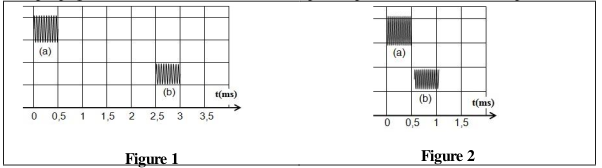
\includegraphics[width=0.22\textwidth]{./img/Ex2.png}
  %\end{center}
%\end{wrapfigure}
Le chlorate de potassium $KClO_3$ est une poudre utilisée dans les feux d'artifice pour obtenir des étincelles violettess
sa réaction avec du carbone (C) donne du dioxyde de carbone $CO_2$ et le chlorure de potassium KCl.

1. Écrire l’équation chimique de la réaction.

2. On réalise la transformation chimique à partir de $n_1$=$1 mol$ de $KClO_3$ et de $n_2$=$1,5 mol$ de carbone.
Construire le tableau d’avancement et déterminer l’avancement final. Indiquer les quantités de chaque espèce dans le
système à l’état final.

3. On réalise la transformation chimique à partir de $25 g$ de $KClO_3$ et de $40 g$ de carbone solides.

3.1. Calculer les quantités de matière initiales des réactifs.

3.2. Construire le tableau d’avancement de la réaction. Déterminer l’avancement maximal de la réaction.

3.3. calculer le volume de dioxyde de carbone gazeux obtenu dans les conditions de l’expérience.

\textbf{Données :}Volume molaire d’un gaz dans les conditions de l’expérience $V_m = 24L/mol$.

Masses molaires atomiques : $M(K)$=$39,1g/mol$ , $M(Cl)$=$35,5g/mol$ , $M(O)$=$16g/mol$ , $M(C)$=$12g/mol$
\end{Box2}

%%_________________________Exercice ! 3:"_________________________Exercice
\begin{Box2}{Exercice 3 :Vitesse de réaction  }
\begin{wrapfigure}{r}{0.5\textwidth}
  \begin{center}
	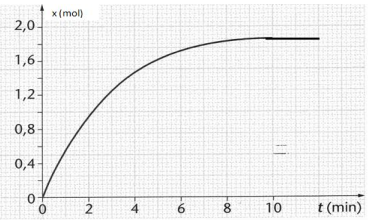
\includegraphics[width=0.5\textwidth]{./img/ex3.png}
  \end{center}
\end{wrapfigure}
La courbe ci-dessous représente les variations de l'avancement x d’une transformation chimique se produisant
en solution aqueuse, en fonction du temps. Le volume V du mélange réactionnel est constant.

\textbf{1. }Justifier l’allure de la courbe en évoquant
l’influence d’un facteur cinétique.

\textbf{2. }Quel est l’avancement final de cette
réaction ?

\textbf{3. }Définir le temps de demi-réaction $t_{1/2}$ et le
déterminer.

\textbf{4. }Dessiner en vert l’allure de la courbe si
l’évolution s’effectuait à une température plus importante. Expliquer.

\textbf{5. }Dessiner en bleu l’allure de la courbe si
l’évolution s’effectuait dans un grand
volume d’eau. Expliquer.
\end{Box2}

%%_________________________Exercice 4 : _________________________Exercice
\begin{Box2}{Exercice 4 : Suivi temporel d’une transformation}
	\begin{wrapfigure}[12]{r}{0.5\textwidth}
  \begin{center}
	  \vspace{-0.6cm}
	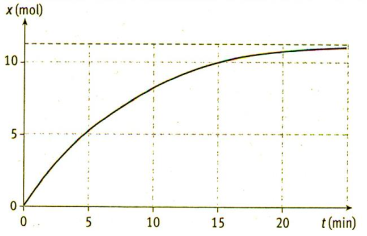
\includegraphics[width=0.5\textwidth]{./img/ex4.png}
  \end{center}
\end{wrapfigure}

	La figure suivante représente la courbe
d'évolution temporelle de l'avancement x
d'une réaction chimique. La transformation
chimique correspondante a été étudiée à une
température constante. Le volume V de
solution est égal à $1,0 L$ et il est constant au
cours de la transformation.

\textbf{1. }Graphiquement, à quoi correspond la vitesse de réaction à un instant t?

\textbf{2. }Calculer $v_0$ la vitesse de réaction à l’instant de date $t_0$ =$0 min$ et $v_1$ celle à l’instant de
date $t_1$=$5min$. Comparer $v_1$ et $v_0$.

\textbf{3. }Comment évolue la vitesse de réaction au cours du temps ? Donner une interprétation de cette variation en envisageant un facteur cinétique.

\textbf{4. }Donner la définition du temps de demi-réaction.

\textbf{5. }Par lecture graphique, déterminer la valeur finale atteinte par l'avancement de la réaction.

\textbf{6. }En déduire la valeur du temps de demi-réaction pour la transformation considérée.

\textbf{7. }Tracer en couleur sur le graphe l’évolution temporelle de l'avancement x pour la même transformation mais
à une température plus élevée.


\end{Box2}
\vspace{-0.8cm}
\begin{center}
   \Large{ \em{Exercices Supplémentaires}}
\end{center}


\vspace{-0.6cm}
%%_________________________Exercice 5 : _________________________Exercice
\begin{Box2}{Exercice 5 :mesurer la quantité d’alcool dans le sang }
Pour mesurer la quantité d’alcool dans le sang, on utilise la réaction chimique suivante :

$3CH_3CH_2OH_{(aq)} + {2Cr_2O_7^{2-}}_{(aq)} + 16H^+_{(aq)} \rightarrow 3CH_3COOH_{(aq)} + 4Cr^{3+}_{(aq)} + 11H_2O_{(l)}$

	\begin{wrapfigure}[14]{r}{0.5\textwidth}
  \begin{center}
	  \vspace{-0.6cm}
	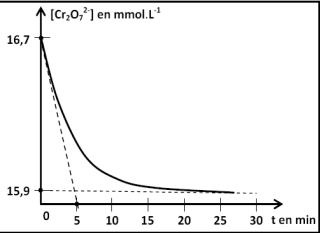
\includegraphics[width=0.5\textwidth]{./img/ex5.png}
  \end{center}
\end{wrapfigure}


Cette réaction est
lente, son évolution est suivie par dosage.

À la date $t = 0$, on mélange $V_p=2mL$ de sang prélevé au bras d’un conducteur avec $V= 10mL$ d’une solution aqueuse acidifiée de dichromate de potassium $(2K^+ + {Cr_2O_7^{2-}}_{(aq)})$ de concentration molaire $C=2.10^{-2} mol.L^{‐1}$.

Le volume total du mélange réactionnel est $V_M$=$12 mL$.

Un suivi temporel obtenu par dosage des ions dichromate $Cr_2O_7^{2-}$ a permis de tracer la courbe suivante.

\textbf{1. }Établir le tableau d’avancement du système en désignant par $n_0$ la quantité de matière initiale
d’alcool présente dans les $2mL$ de sang, et par $n_1$ la quantité de matière initiale en ions dichromate introduite dans le mélange réactionnel. (L’ion $H^+$ est en excès).

\textbf{2. }Quelle relation existe entre l’avancement x de la réaction, la concentration en ions dichromate $[Cr_2O_7^{2-}]$ dans le mélange, le volume $V_M$ du mélange réactionnel, et la quantité $n_1$ ?

\textbf{3. }La réaction peut être considérée comme
totale. À l’aide du graphique $[Cr_2O_7^{2-}]$ =$ f(t)$,
calculer l’avancement maximal.

\textbf{4. }Le taux autorisé d’alcool est de 0,5 g dans 1 L
de sang. Le conducteur est‐il en infraction ?

\textbf{5. }Donner la définition de la vitesse de la
réaction.

\textbf{6. }Déterminer sa valeur à l’instant initial.

\textbf{Données : Masse molaire moléculaire de l’éthanol 46g/mol}

\end{Box2}


\end{document}
